\chapter{Methodology\label{cha:chapter4}}
As discussed in \autoref{cha:chapter2}, learning-based compression of \ac{rgb} imagery is a hot topic in current research. Therefore, being able to use and further research methods used in that field for hyperspectral image compression would be useful. However, direct application of most learning-based \ac{rgb} image compression methods on hyperspectral data is not possible. This is mainly for two reasons. Firstly, learning-based \ac{rgb} image compression methods ignore dependencies between the three channels in the \ac{rgb} images and focus solely on spatial dependencies. This is useful for \ac{rgb} images because the spectral dependencies within the three channels are low, since the corresponding wavelengths are far apart. Additionally, having only three channels means that there is not much spectral information per pixel to be compressed, meaning that even if spectral dependencies existed, the compression gains that could be extracted would be small. This is different in hyperspectral image compression where there are large amounts of spectral dependencies and the potential compression gains are much larger because of the high number of spectral channels. It is therefore necessary to modify \ac{rgb} models to incorporate spectral dependencies in order to adapt them to the task of hyperspectral image compression. 

The second reason for the difficulty in applying \ac{rgb} image compression methods to hyperspectral images is the significant increase in spectral dimension. Compared to an \ac{rgb} image, a hyperspectral image of the same size with 200 channels has $200/3 \approx 67$ times more dimensions. For this reason \ac{rgb} models are often too small to learn the compression of high-dimensional hyperspectral image data. For example, many \ac{cnn} models use an input layer transforming the input from the dimensions $H \times W \times C$, where $H$ and $W$ are the height and width and $C$ is the number of channels to $H' \times W' \times N$, where $H'$ and $W'$ are often either the original height and width or half the original height and width and $N$ is the number of filters used in the input layer. If $H'$ and $W'$ are equal to half the original height and width, this is achieved either using a pooling layer or a convolutional layer with a stride of two. In \ac{rgb} models, 128 and 192 are common values for $N$. For \ac{rgb} images, this means that the input layer increases the dimensionality drastically in order to learn multiple features of the image. However, in hyperspectral images, the same layer would result in a decrease of dimensionality leading to a loss of information. A simple approach to address this issue is to increase the number of filters in each layer according to the increase in dimensionality between \ac{rgb} and hyperspectral images. The input layer would then for example have $192 * 67 = 12864$ filters. However, this would result in a much larger model than the corresponding \ac{rgb} compression model and therefore require a higher amount of computational resources for training, potentially making the model impossible to train on the available hardware. Additionally, even if the models were trainable, it is unclear if the convolutional layer would be able to learn such a high amount of distinct features for hyperspectral images.

Therefore, a different model architecture is required. This thesis presents a novel architecture that allows the use of spatial compression methods designed for an almost arbitrary number of channels in hyperspectral image compression while also incorporating spectral dependencies. This not only allows the use of \ac{rgb} image compression methods but also multispectral compression methods. The proposed architecture is called "Combined Model" and an overview is shown in \autoref{fig:combined}.
%Furthermore, it is also possible to use non-learning-based methods using a desired number %of channels, like \ac{jpeg} 2000, on hyperspectral data while integrating spectral %dependencies of hyperspectral images. 
\section{The Combined Model\label{sec:combinedmodel}}
\begin{figure}
\centering
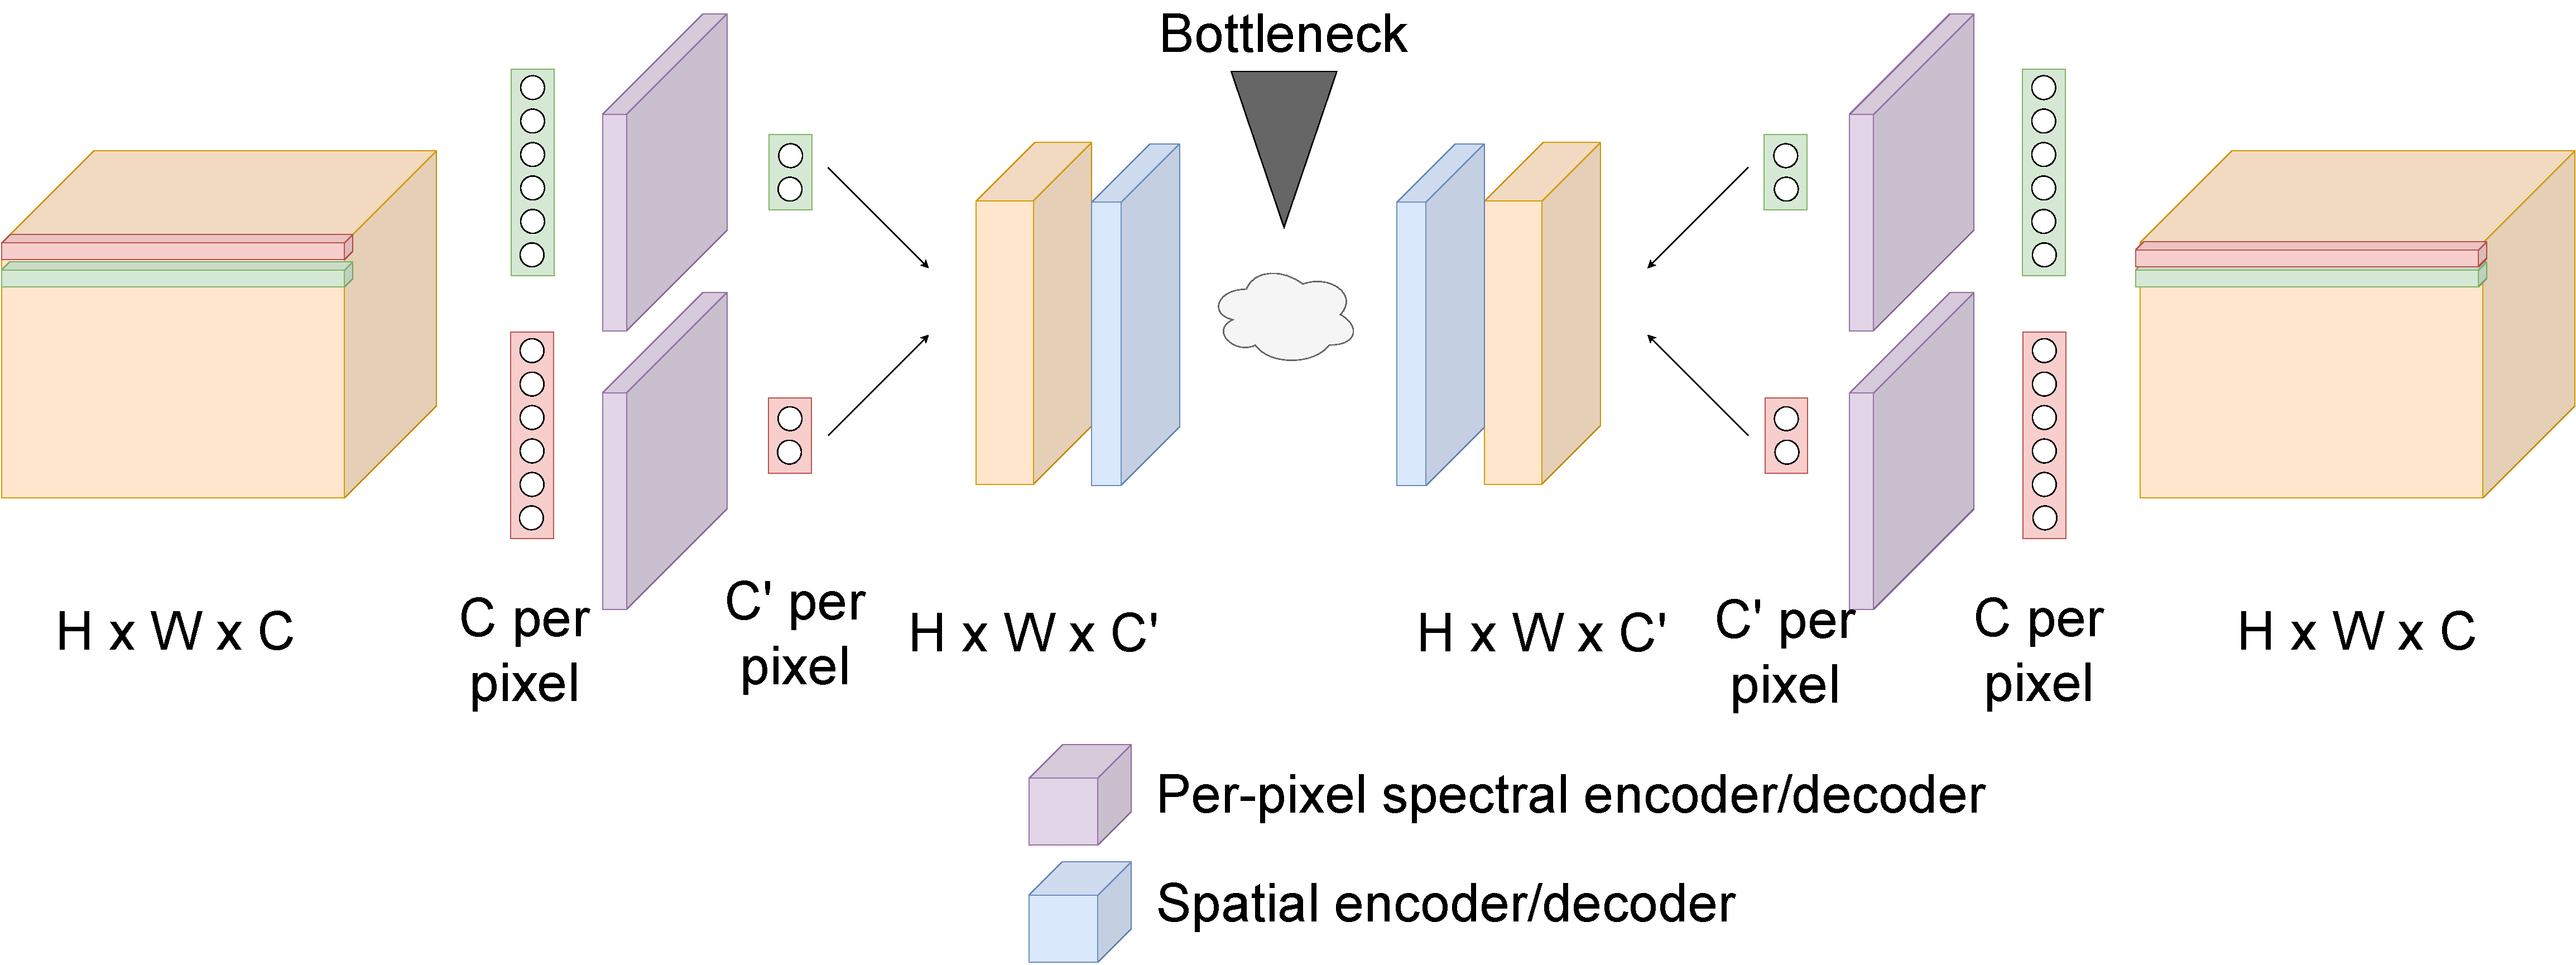
\includegraphics[scale=0.18]{img/GeneralArchitecture.pdf}
\caption[Combined model architecture]{Architecture of the Combined Model using the per-pixel spectral \ac{cnn}}
\label{fig:combined}
\end{figure}

The main idea of the combined model is to use a spectral encoder network that preserves spatial dependencies in order to reduce the number of spectral channels in the input. Then, a spatial compression method is applied on the output of that spectral encoder in order to exploit the spatial dependencies. The resulting bottleneck is then decoded using the corresponding spatial decoder. Finally, a spectral decoder network symmetrical to the spectral encoder restores the original image. During training, the spectral decoder learns to adapt to the distortion introduced by the spatial autoencoder. If the spatial autoencoder is learning-based, it similarly learns to produce an output in such a way that the spectral autoencoder can decode it more effectively. The corresponding mechanism is studied in detail in \autoref{cha:chapter5}. Adaptation in either the spatial autoencoder or the spectral autoencoder are necessary, especially if the latent space of the spectral autoencoder is not continuous. In that case, a small change introduced by the spatial autoencoder could result in a large change in the output of the spectral decoder. In practice the adaptation process is successful in avoiding chaotic outputs of the spectral decoder, which is also shown in \autoref{cha:chapter5}.

The aforementioned approach has multiple advantages. It is highly flexible with regard to the spatial autoencoder. Many different learning-based approaches can be used and the number of input channels to the spatial autoencoder can be modified so it best fits the spatial autoencoder. This can be achieved by modifying the compression ratio of the spectral encoder/decoder pair, which is possible for all spectral autoencoder models studied in this thesis. Another advantage is that the distinct separation between the spatial and the spectral encoding allows for informative studies to be done both regarding explainability and regarding the amount of spatial and spectral dependencies in the data. The model also allows for different spectral encoder and decoder architectures. There are two necessary conditions required for a spectral encoder/decoder pair to be possible for use in the combined model. Firstly, the output of the encoder must be an image-like shape in order for spatial image compression models to be used for incorporating the spatial dependencies. Secondly, the spectral encoder needs to preserve spatial dependencies, ideally resulting in an output with similar spatial dependencies to the actual input image. Because the spatial autoencoder models were designed for image compression, having spatial dependencies close to the dependencies found in images means that the task the spatial autoencoder is used for is close to the one it was designed for.

However, a difference between the task of image compression and the task the spatial autoencoder performs, that being compression of the latent of the spectral autoencoder, is still present. This is one of the disadvantages of the combined model approach and therefore requires the spatial autoencoder to be resilient to this change of task. However, for the spectral autoencoder models studied in this thesis, the spatial dependencies of the latents very closely resemble the spatial dependencies of the original input, mitigating this disadvantage. For further detail on this see \autoref{cha:chapter5}.

For training the Combined Model, an additional idea is useful. If the model is trained in a standard way by training both the spatial autoencoder and the spectral encoder/decoder pair end-to-end from a newly initialized state at the same time, the results can be unstable. Depending on the hyperparameters, it may not be possible to train the combined model in this way. This follows from the fact that inputs to the spatial autoencoder depend on the outputs of the spectral encoder. During the start of training, the spectral encoder often outputs similar or equal values for all inputs. The spatial autoencoder may then specifically learn to compress latents with these specific values, which is a task very different from compressing spatial dependencies. In this case, the dependencies between the model parts can inhibit training and lead to the model being stuck in the local minimum of outputting the same output for any input. We solve this problem by pretraining the spectral encoder/decoder pair as an autoencoder without any spatial component. Then the combined model is trained using the pretrained spectral encoder and decoder. In this way, the spatial autoencoder receives useful input data from the beginning of training. 

An interesting modification option for the model follows from pretraining the spectral encoder/decoder pair. After pretraining the spectral component, the combined model can be trained while freezing the spectral component, training only the spatial autoencoder. If trained in this way, the combined model can be seen as a spatial image compression model using an involved preprocessing and postprocessing step. This option is analysed and compared with the normal method of training the combined model in \autoref{cha:chapter5}.
\section{Spectral Autoencoder Methods}
Three different architectures were studied for the spectral encoder and decoder models. Firstly, we analysed a per-pixel \ac{cnn} using one-dimensional convolutional layers on the spectral domain of the hyperspectral images. We then developed another \ac{cnn}-based model using two-dimensional convolutional layers to address some of the disadvantages of the one-dimensional \ac{cnn} approach. Finally, we studied the possibility of directly using a \ac{vae} for compression of the spectral information in hyperspectral images. 
\subsection{Per-Pixel Convolutional Neural Network\label{sec:conv1d}}
\begin{figure}
\centering
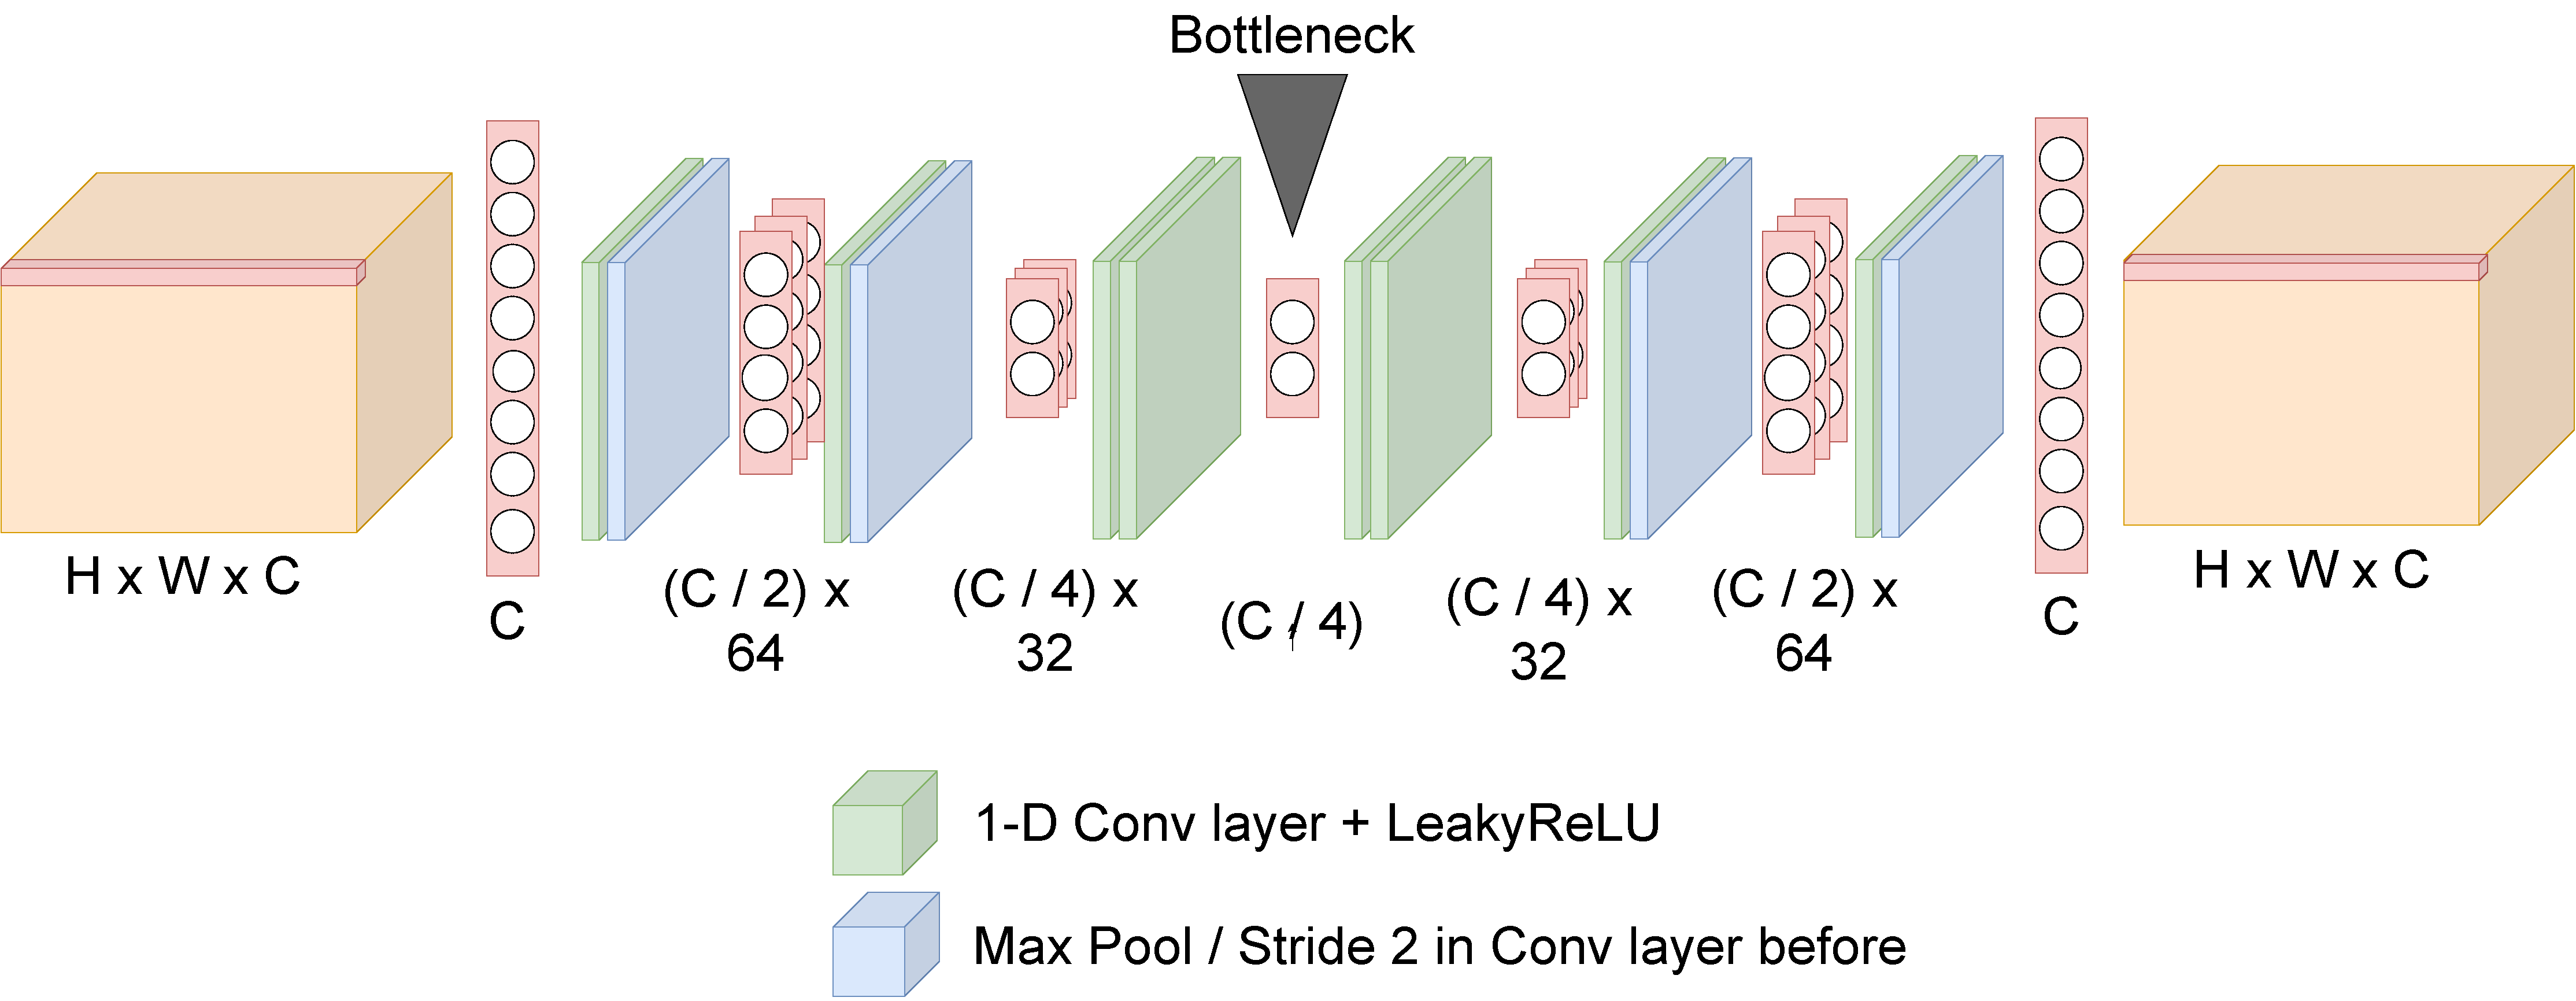
\includegraphics[scale=0.18]{img/OneDCNN.pdf}
\caption[Per-Pixel spectral \ac{cnn}]{Architecture of the per-pixel spectral \ac{cnn} using two downsampling layers resulting in a compression factor of four}
\label{fig:onedcnn}
\end{figure}
The first of the spectral autoencoder methods is based on the model proposed by Kuester et.al. \citep{kuester_1d-convolutional_2021,kuester_transferability_2022}. In their proposed method a hyperspectral input is split up into its pixels. The spectrum for each pixel then forms one datapoint on which the model is trained. The encoder of the model being trained is a \ac{oned} \ac{cnn} consisting of two sets of a \ac{oned} convolutional layer with a large kernel size of 11 and a max pooling layer followed by two additional \ac{oned} convolutional layers with a kernel size of 9 and 7. The number of filters is also reduced by a factor of two in each convolutional layer and set to one in the last layer, resulting in a bottleneck with one fourth of the original spectral channels. The decoder is built analogously, only replacing the max pooling layers by upsampling layers. After each convolutional layer a \ac{lrelu} is used as the activation function. Additionally, the number of channels are padded with channels containing zero values in order for them to be divisible by the downsampling factor of 2. Since the number of channels is reduced by a factor of twice the downsampling factor during encoding, this can result in the bottleneck not having exactly one fourth of the channels of the input, if the number of channels in the padded input is not divisible by four. The decoder then outputs one channel more than the original input. In this case, the last channel of the output is removed. A whole image can be compressed by encoding and decoding each pixel of the image separately, then reassembling the output image from the decoded pixels. The architecture of this model is shown in \autoref{fig:onedcnn}.

This model is highly compatible with the Combined Model approach. Because the encoding of the spectral channels is performed per pixel, spatial dependencies are guaranteed to remain during encoding. The latent image is produced similarly to the output of the decoder by reassembling the latents for each pixel into a latent image, which can then be further encoded using a spatial autoencoder. In order to optimize the model for use in the combined model architecture and for the used dataset HySpecNet-11k \citep{fuchs_hyspecnet-11k_2023}, we adapted the model in various ways.

In the model as proposed by Kuester et.al. \citep{kuester_1d-convolutional_2021,kuester_transferability_2022}, the number of layers and therefore the compression ratio is fixed to four. However, different datasets can have different amounts of spatial and spectral dependencies. For of the Combined Model, this can result in the optimal model requiring a different spectral compression factor than 4. To allow for a different compression ratio, the number of sets of a convolutional and a max pooling layer was enabled to be variable. In addition to this, the number of filters in each convolutional layer was adapted to the number of channels in the data. In the original paper, the first layer has a number of filters equal to half the number of padded channels of the data. We adapted the number of filters to the higher number of channels in the HySpecNet-11k dataset by keeping this ratio equal. We thereby ensure that the number of filters is always appropriately divisible regardless of the number of layers by performing the padding on the spectral channels of the input. We also changed the padding strategy. Instead of padding to a number of spectral channels divisible by half the compression ratio and then conditionally removing some number of channels at the output, we directly padded to a number of spectral channels divisible by the compression ratio. Therefore the need for removing channels at the output is removed, simplifying the model without loss of performance.

The spectral compression model is not only interesting for its applicability to the combined model. It is also the hyperspectral compression model with the highest reconstruction accuracy for multiple bitrates among many compared models. For more on this see \autoref{cha:chapter5}. However, there are also some disadvantages of the model architecture. The reduction of spectral channels using max pooling layers results in divisions by two in the number of channels, forcing the compression ratio to be a power of two. Additionally, the higher the chosen compression ratio is, the higher the number of needed padding channels is. As an example, for the HySpecNet-11k dataset with 202 channels two padding channels are needed for the compression ratio 4, for a compression ratio of 32 14 padding channels would be required. Finally, the training process of this model is much slower than the training process for models which take complete images as input. Since each pixel is compressed separately, the number of optimization steps per epoch is much higher. This is also further discussed in \autoref{cha:chapter5}.
\subsection{Two-dimensional Spectral CNN\label{sec:fastconv1d}}
To address the issues of the \ac{oned} spectral \ac{cnn}, we propose another model that uses \ac{twod} convolutional layers with a kernel size of one to compress a whole image at once. For convolutional layers with a kernel size of one the convolution operation collapses down to a scalar multiplication. Additionally, the output has the same height and width as the input, as each pixel in the output is calculated only from the channels of a corresponding input pixel. The output for a specific pixel and filter is therefore equivalent to a weighted sum over all channels in the input for this pixel. Importantly however, the weight used for a specific input channel is the same for each pixel in the image. A two-dimensional convolutional layer with a kernel size of one can therefore only encode spectral information when applied to a hyperspectral image, making it usable as part of the Combined Model. Such layers are commonly used for decreasing the number of filters between other convolutional layers TODO REF. Because of this, they are also referred to as channel or feature map pooling layers. They are then able to learn non-trivial summarizations of the preceding layer because of the nonlinearity introduced by the used activation function, in our case \ac{lrelu}. However, they can also instead be used to achieve the opposite effect of increasing the number of filters while retaining the semantic information within these filters. An example of both of these uses is present in the "Inception" architecture proposed in Szegedy et.al. \citep{szegedy_going_2014}.

We show that it is also possible to use such layers to learn spectral dependencies in hyperspectral image data. The model is comprised of two-dimensional convolutional layers starting with a number of filters slightly higher than the number of channels in the hyperspectral dataset the model is trained on, which is 256. In each layer, the number of filters is doubled in order to increase the amount of information available. Finally, a last convolutional layer is used to reduce the number of channels to result in the desired bottleneck size. All convolutional layers use a kernel size of one and the \ac{lrelu} activation function.

The \ac{twod} architecture has multiple advantages compared with the one-dimensional spectral \ac{cnn}. Instead of being applied per pixel, it can be applied to the entire image at the same time. It also requires less parameters, as each layer has a number of parameters equal to $N_p = C * F$, where $C$ is the number of channels of the input to the layer and $F$ is the number of filters in the layer. Both of these factors result in a much shorter training time as seen in \autoref{cha:chapter5}. The model is also more flexible with regard to the compression ratio. In contrast to the one-dimensional spectral encoder, where the compression ratios are necessarily given by $R \approx 2^N$, where $N$ is the number of pooling layers, the two-dimensional spectral encoder allows setting of the number of output channels to an arbitrary number. This also removes the need for padding, which is an advantage especially for high compression ratios which would otherwise require padding. Furthermore, the one-dimensional spectral \ac{cnn} gets slower for higher compression ratios as it requires more layers while the number of layers and therefore the speed of the two-dimensional spectral \ac{cnn} is constant with respect to the compression ratio.

Two modifications were also tested for this model. First, a Layer Normalization was performed after each convolutional layer in order to improve generalization performance and further reduce training time.  We also modified the model by changing the kernel sizes of the convolutional layers. With higher kernel sizes, the model becomes able to incorporate some amount of local spatial dependencies in addition to the spectral dependencies. We used this to study how sensitive the combined model is to spatial dependencies being partially encoded in the spectral encoder/decoder.
\subsection{Variational autoencoder \label{sec:vae}}
As mentioned in \autoref{sec:combinedmodel}, a requirement for spectral encoder / decoder pair is that the decoder is able to decode the latent of the encoder after some distortion  has been to it applied by the spatial autoencoder. Therefore, using a \ac{vae} for the spectral compression is potentially advantageous, because \acp{vae} produce a continuous latent space as shown by TODO REF. A \ac{vae} learns a probability distribution for a latent space and produces reconstructions by generating a samples from this distribution. We designed a one-dimensional \ac{vae} with the purpose of learning to autoencode spectral dependencies for single pixels, similar to the per-pixel \ac{cnn}. This per-pixel \ac{vae} in fact uses the per-pixel \ac{cnn} to produce a latent for a given input pixel. Two independent linear layers are then applied to this latent to produce a mean and a variance tensor respectively. The dimensionality of these vectors is variable and therefore a hyperparameter of the model. The linear layer producing the mean uses a tanh activation function to constrain the means between -1 and 1. The linear layer producing the variance also uses tanh but follows by an application of the softplus function to produce a positive variance. A new latent is then sampled from this distribution to produce the input for the decoder which is a symmetric inverted version of the encoder with only one linear layer instead of two, since only the new latent needs to be transformed to the latent space of the per-pixel \ac{cnn}.

A basic \ac{vae} has not previously been used for hyperspectral image compression. Especially compression of spectral signatures using a one-dimensional \ac{vae} has not been studied. The only \acp{vae} architecture commonly used for image compression is the hyperprior architecture, which is described in \autoref{cha:chapter4}. However, these models are not applicable to be a spectral autoencoder for the Combined Model for two reasons. First, hyperprior models so far have been used for spatial dependencies in images, being applied to whole images at once and not one-dimensionally to spectral signatures. Secondly, since hyperprior models use an arithmetic coder in the bottleneck, they can only be used as the last stage of a compression model since the output of the arithmetic coder cannot be further compressed using another model. This model attempts to overcome these limitations to produce a continuous latent space that can be further compressed using a spatial autoencoder method while being permissible with regard to distortions being introduced during this process.
\section{Spatial Autoencoder Methods\label{sec:spatialae}}
The second part of the Combined Model is the spatial autoencoder that further compresses the bottlneck of the spectral encoder. While there are some preconditions required for the spectral encoder/decoder pair, the choice of the spatial autoencoder is highly flexible. Since the latents of the spectral encoder have similar spatial dependencies to actual images, any autoencoder that is able to compress images can be used for this part of the model. The models analysed in this thesis are a \ac{cnn}-based autoencoder, a hyperprior model and an optimized hyperprior model using self-attention modules and a context model. We also analysed the use of \ac{jpeg} 2000 as the spatial autoencoder to study the viability of using a spatial autoencoder as part of the combined model that is not learning-based.
\subsection{CNN-based Spatial Autoencoder\label{sec:conv2d}}
The \ac{cnn}-based spatial autoencoder model uses a low-complexity approach using only two-dimensional convolutional layers. A similar architecture was used for hyperspectral image compression by La Grassa et.al. \citep{la_grassa_hyperspectral_2022}. However, there are multiple differences between the model. La Grassa et.al. use a linear layer as the final layer of their network. This was not done for the \ac{cnn}-based spatial autoencoder as it would increase the number of parameters of the model and therefore increase both training time and the required computational resources. The model proposed in this thesis also adds regularization into the model using layer normalization \citep{ba_layer_2016}. The number of filters in each layer is also different. Further, La Grassa et.al. use max pooling layers to reduce the spatial dimensionality of the latent while we use convolutional layers with a stride. Additionally, we experiment with different kernel sizes to vary the amount of spatial dependencies introduced to the autoencoder.

The \ac{cnn}-based spatial autoencoder model first uses two-dimensional convolutional layers to increase the dimensionality of an input image. This is done by using a number of filters much higher than the number of channels in the input. This input layer is followed by another convolutional layer with the same number of filters to increase the depth of the model. Following that is a convolutional layer with a stride of two to reduce the spatial dimensions. This layer also increases the number of filters in order to reduce the information loss while downsampling. Finally, two further convolutional layers reduce the filter dimension to be identical to the number of channels in the input. In this way the dimensionality of the input is reduced by a factor of two in each spatial dimension, resulting in an overall compression factor of four. Additional layers with a stride of two can be added to increase the compression factor. The decoder is symmetrical to the encoder but replaces convolutional layers with transposed convolutional layers. The model uses the \ac{prelu} activation function after each convolutional layer and the sigmoid activation function after the final layer of the encoder and the decoder to keep outputs in the interval $[0,1]$. Layer normalization \citep{ba_layer_2016} is also performed after each convolutional layer to increase robustness and rate of convergence during training. Layer normalization was used instead of the more common batch normalization because it is able to perform well even with a low batch size and the combined model with the per-pixel \ac{cnn} was trained using a batch size of one.

This model was deliberately designed to be low-complexity to reduce the confounding factors for studying properties of the combined model. As there is no prior research for combining models in the way it was performed in this thesis for hyperspectral or \ac{rgb} image compression, the properties of the combined architecture as a whole was a focus of the experiments. A low-complexity spatial model is therefore a useful baseline that allows for better attribution of specific experimental results to the combined architecture.
\subsection{Hyperprior-based Spatial Autoencoder}
To also include a more complex model with high relevancy in \ac{rgb} compression research, we implemented the scale hyperprior model proposed by Ballé et.al. \citep{balle_end--end_2017}. Since this model was explored in detail in \autoref{cha:chapter4}, we will not go into further detail here. The only necessary adaptation to the model in order to use it as part of the Combined Model was a change of the input and output layer to accommodate the chosen number of channels in the latent of the spectral encoder. This model was not studied intensively but rather used as a baseline. The main hyperprior-based architecture used was the following model using self-attention modules and a context model.
\subsection{Attention-based Model Using Hyperprior Architecture\label{sec:atthyperprior}}
The main hyperprior-based model that was studied is based on work by Cheng et.al. \citep{cheng_learned_2020}. They further improve the joint autoregressive and hierarchical hyperprior model by Minnen et.al. \citep{minnen_joint_2018} discussed in detail in \autoref{cha:chapter4} by introducing self-attention modules. The attention modules are based on work by Liu et.al. \citep{liu_non-local_2019}. However, the non-local blocks have been removed in order to simplify the attention modules. This allowed them to reduce the complexity of the model while still being able to adequately capture long-range dependencies in the data. These self-attention modules were inserted into the main encoder and decoder in two places as shown in Fig. TODO.

We adapted this model in multiple ways for use in the combined model. First, the model was adapted to be able to receive different numbers of input channels by changing the input and output layers. The second modification regards the strength of the spatial downsampling in the convolutional parts of the hyperprior model. In the original model the main encoder reduces the spatial dimensionality by a factor of 8 in each direction, 64 in total, to produce the latent that is input to both the arithmetic coder and the hyperprior encoder. The hyperprior encoder reduces the spatial dimensions by a factor of 4 in each direction, 16  total, again. Since they used a dataset with 256x256 pixels, this results in a bottleneck of size 32x32 after the main encoder and 8x8 after the hyperprior encoder. However, for hyperspectral data in general and the HySpecNet-11k dataset especially a reduction in spatial dimension with a factor of 64 can result in large distortion, since there are less spatial dependencies than in typical \ac{rgb} datasets. We therefore modified both the numbers of convolutional layers and the strides in the main encoder/decoder pair and the hyperprior encoder/decoder pair in order to allow for different options for the spatial dimensionality reduction factors. For this, we group models by the spatial reduction factors in the main encoder/decoder pair and the bottleneck size of the hyperprior encoder. The bottleneck size of the hyperprior being larger results in more information remaining present in the hyperprior which increases performance. However, more side information needs to be transmitted, which can decrease performance. This is because the loss used for training these models, \ac{rd} loss, tries to achieve a balance between bitrate and distortion. Since a larger amount of transmitted side information raises bitrate, \ac{rd} loss with the same parameters will also result in higher distortion. Therefore, an optimum needs to be found depending on the amount of spatial dependencies present in the dataset.